\chapter{Method}
\label{chap:partI_methods}

This work tackles the problem of segmenting and counting cells in a \textit{supervised learning} framework. For this purpose, we address the segmentation task exploiting four CNN architectures belonging to the Unet and ResUnet families. 
Once the cells are detected, the final count is retrieved as the number of connected pixels in the post-processed output.
In doing so, we also test the impact of study design choices intended to reduce false negatives and promote accurate segmentation.

\section{Model architecture}
\label{model_architecture}

\begin{figure}
\centerline{
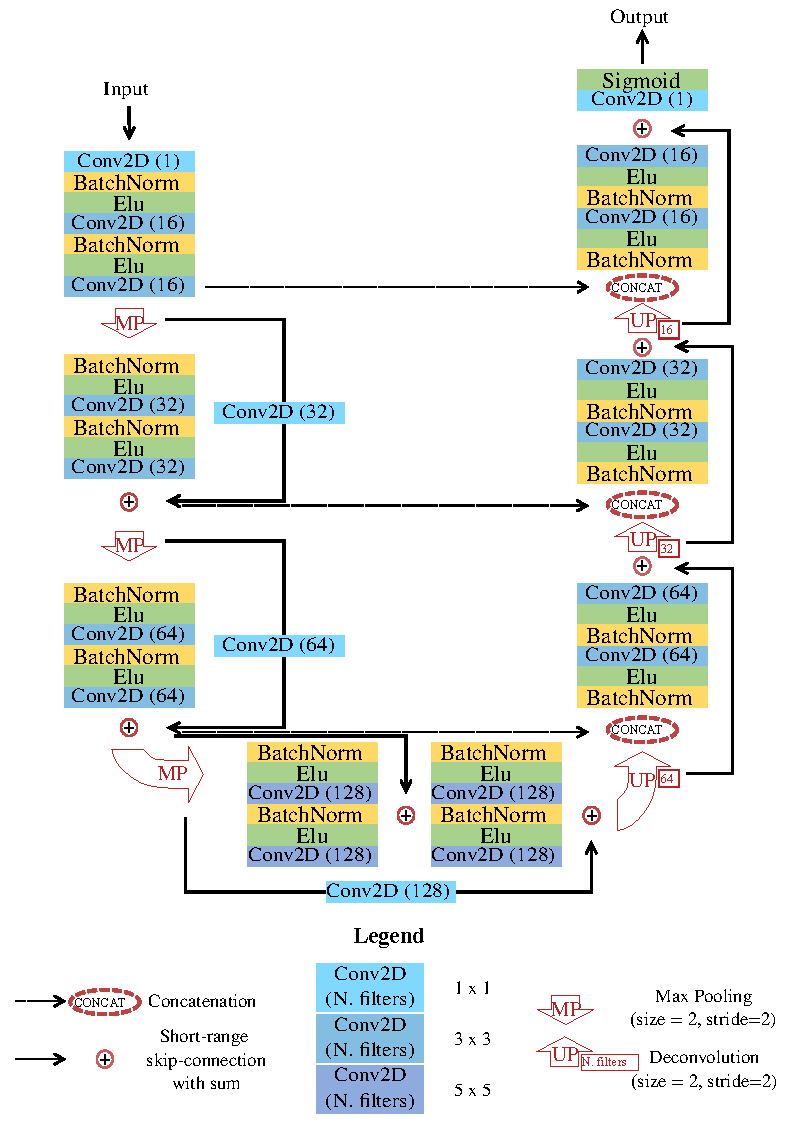
\includegraphics[width=0.8\textwidth]{figures/130_methods/c-resunet_architecture.pdf}
}
\caption{\textbf{Model architecture}. Each box reports an element of the entire architecture (individual descriptions in the legend). 
% The shortcut-connections along the encoding-path are supported by a 1$\times$1 convolution to enable the final sum before the max-pooling operation.
} \label{fig:model_architecture}
\end{figure}
We compare the detection and counting performance of four alternative architectures derived from two network families, Unet and ResUnet, commonly used for segmentation tasks.
In the former family, we pick the original Unet architecture \cite{unet} and a smaller version (small Unet) obtained by setting the initial number of filters equal to the ResUnet proposed in Zhang et al. \cite{deep_resunet} and scaling the following blocks consequently.
In the latter, we pick a ResUnet implementation available in literature \cite{deep_resunet} and a similar version with minor modifications.
Specifically, we add an initial 1$\times$1 convolution to simulate an RGB to grayscale conversion which is learned during training.
Moreover, we insert an additional residual block at the end of the encoding path with 5$\times$5 filters (instead of 3$\times$3). These adjustments should provide the model with a larger field of view, thus fostering a better comprehension of the context surrounding the pixel to classify.
This kind of information can be beneficial, for example, when cells clump together and pixels on their boundaries have to be segmented. 
Likewise, the analysis of some background structures (Fig. \ref{fig:dataset}, top-left image) can be improved by looking at a broader context.
The resulting architecture is reported in Fig. \ref{fig:model_architecture} and it will be referred to as \textbf{cell ResUnet (c-ResUnet)} hereafter.

\section{Ablation studies}
\label{sec:ablation_studies}

Alongside the four network architectures, we also tested the effect of two design choices intended to mitigate errors on challenging images containing artifacts and cells overcrowding.

\noindent\textbf{Artifacts Oversampling (AO)}. 
The presence of biological structures or artifacts like those in Fig. \ref{fig:dataset} (rightmost pictures) can often fool the model into detecting false positives. Indeed, their similarity with cells in terms of saturation and brightness, added to the fact that they are underrepresented in the data, make it difficult for the model to handle them correctly.
For this reason, we tried to increase the augmentation factor for these inputs to facilitate the learning process. Specifically, we selected 6 different crops representing such relevant structures and re-sampled them with the augmentation pipeline described in \textit{Model training}, resulting in 150 new images for each crop. 
% The transformations applied regarded rotations, addition of gaussian noise, elastic transformation and brightness, hue, saturation variation.

\noindent\textbf{Weight Maps (WM)}. \label{sec:weights_map}
One of the toughest challenges during the inference is related to cell overcrowding. 
As a matter of fact, failing to precisely segment cells boundaries may lead to spurious connections between objects that are separated. Consequently, multiple objects are considered as a single one and the model performance deteriorates.
In order to improve cell separation, Ronneberger et al. \cite{unet} suggested leveraging a weight map that penalizes more the errors on the borders of touching cells.
Building on that, we introduce a novel implementation where single object contributions are compounded additively.
This procedure generates weights that decrease as we move away from the borders of each cell. 
At the same time, the contributions coming from single items are combined so that the global weight map presents higher values where more cells are close together (\mbox{see Fig. \ref{fig:weight_calculation}}).
\begin{figure}
\centerline{
     \begin{subfigure}[]{0.4\textwidth}
         \centering
         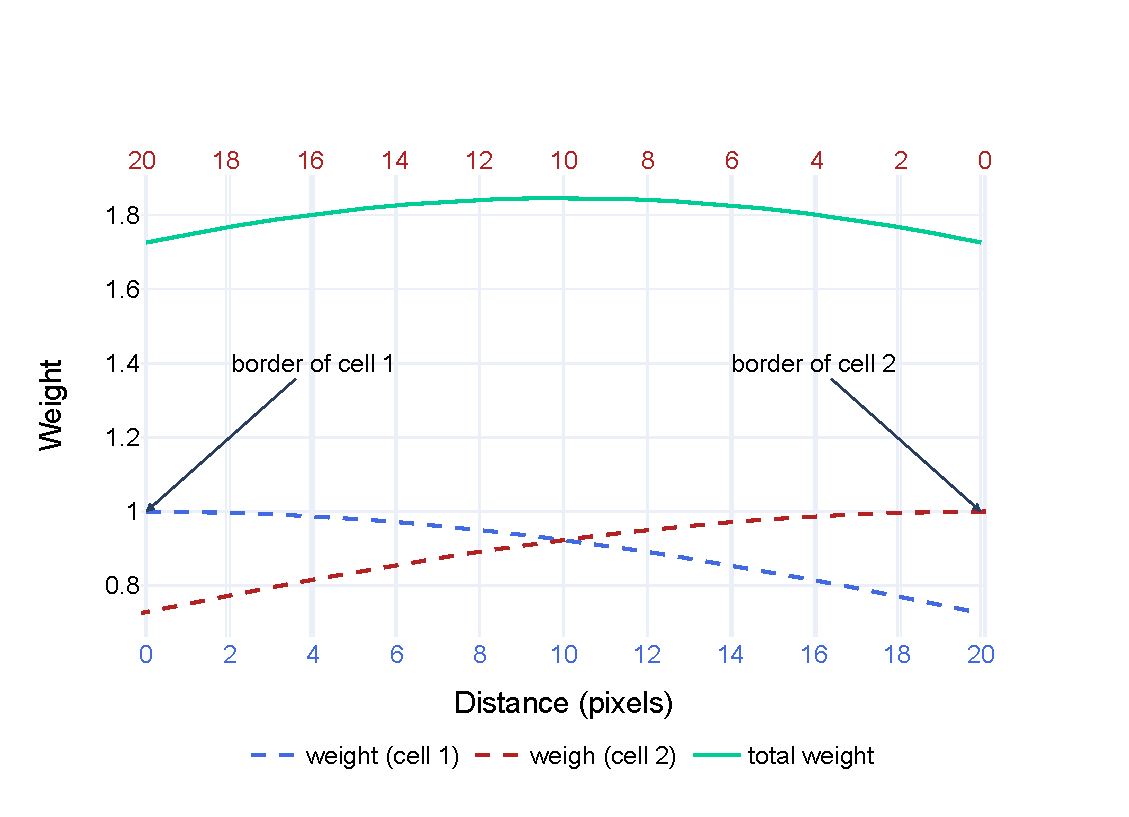
\includegraphics[width=\textwidth]{figures/130_methods/weight_calculation.eps}
        \caption{Weight compounding}
        \label{fig:weight_calculation}
     \end{subfigure}
     \begin{subfigure}[]{0.62\textwidth}
         \centering
         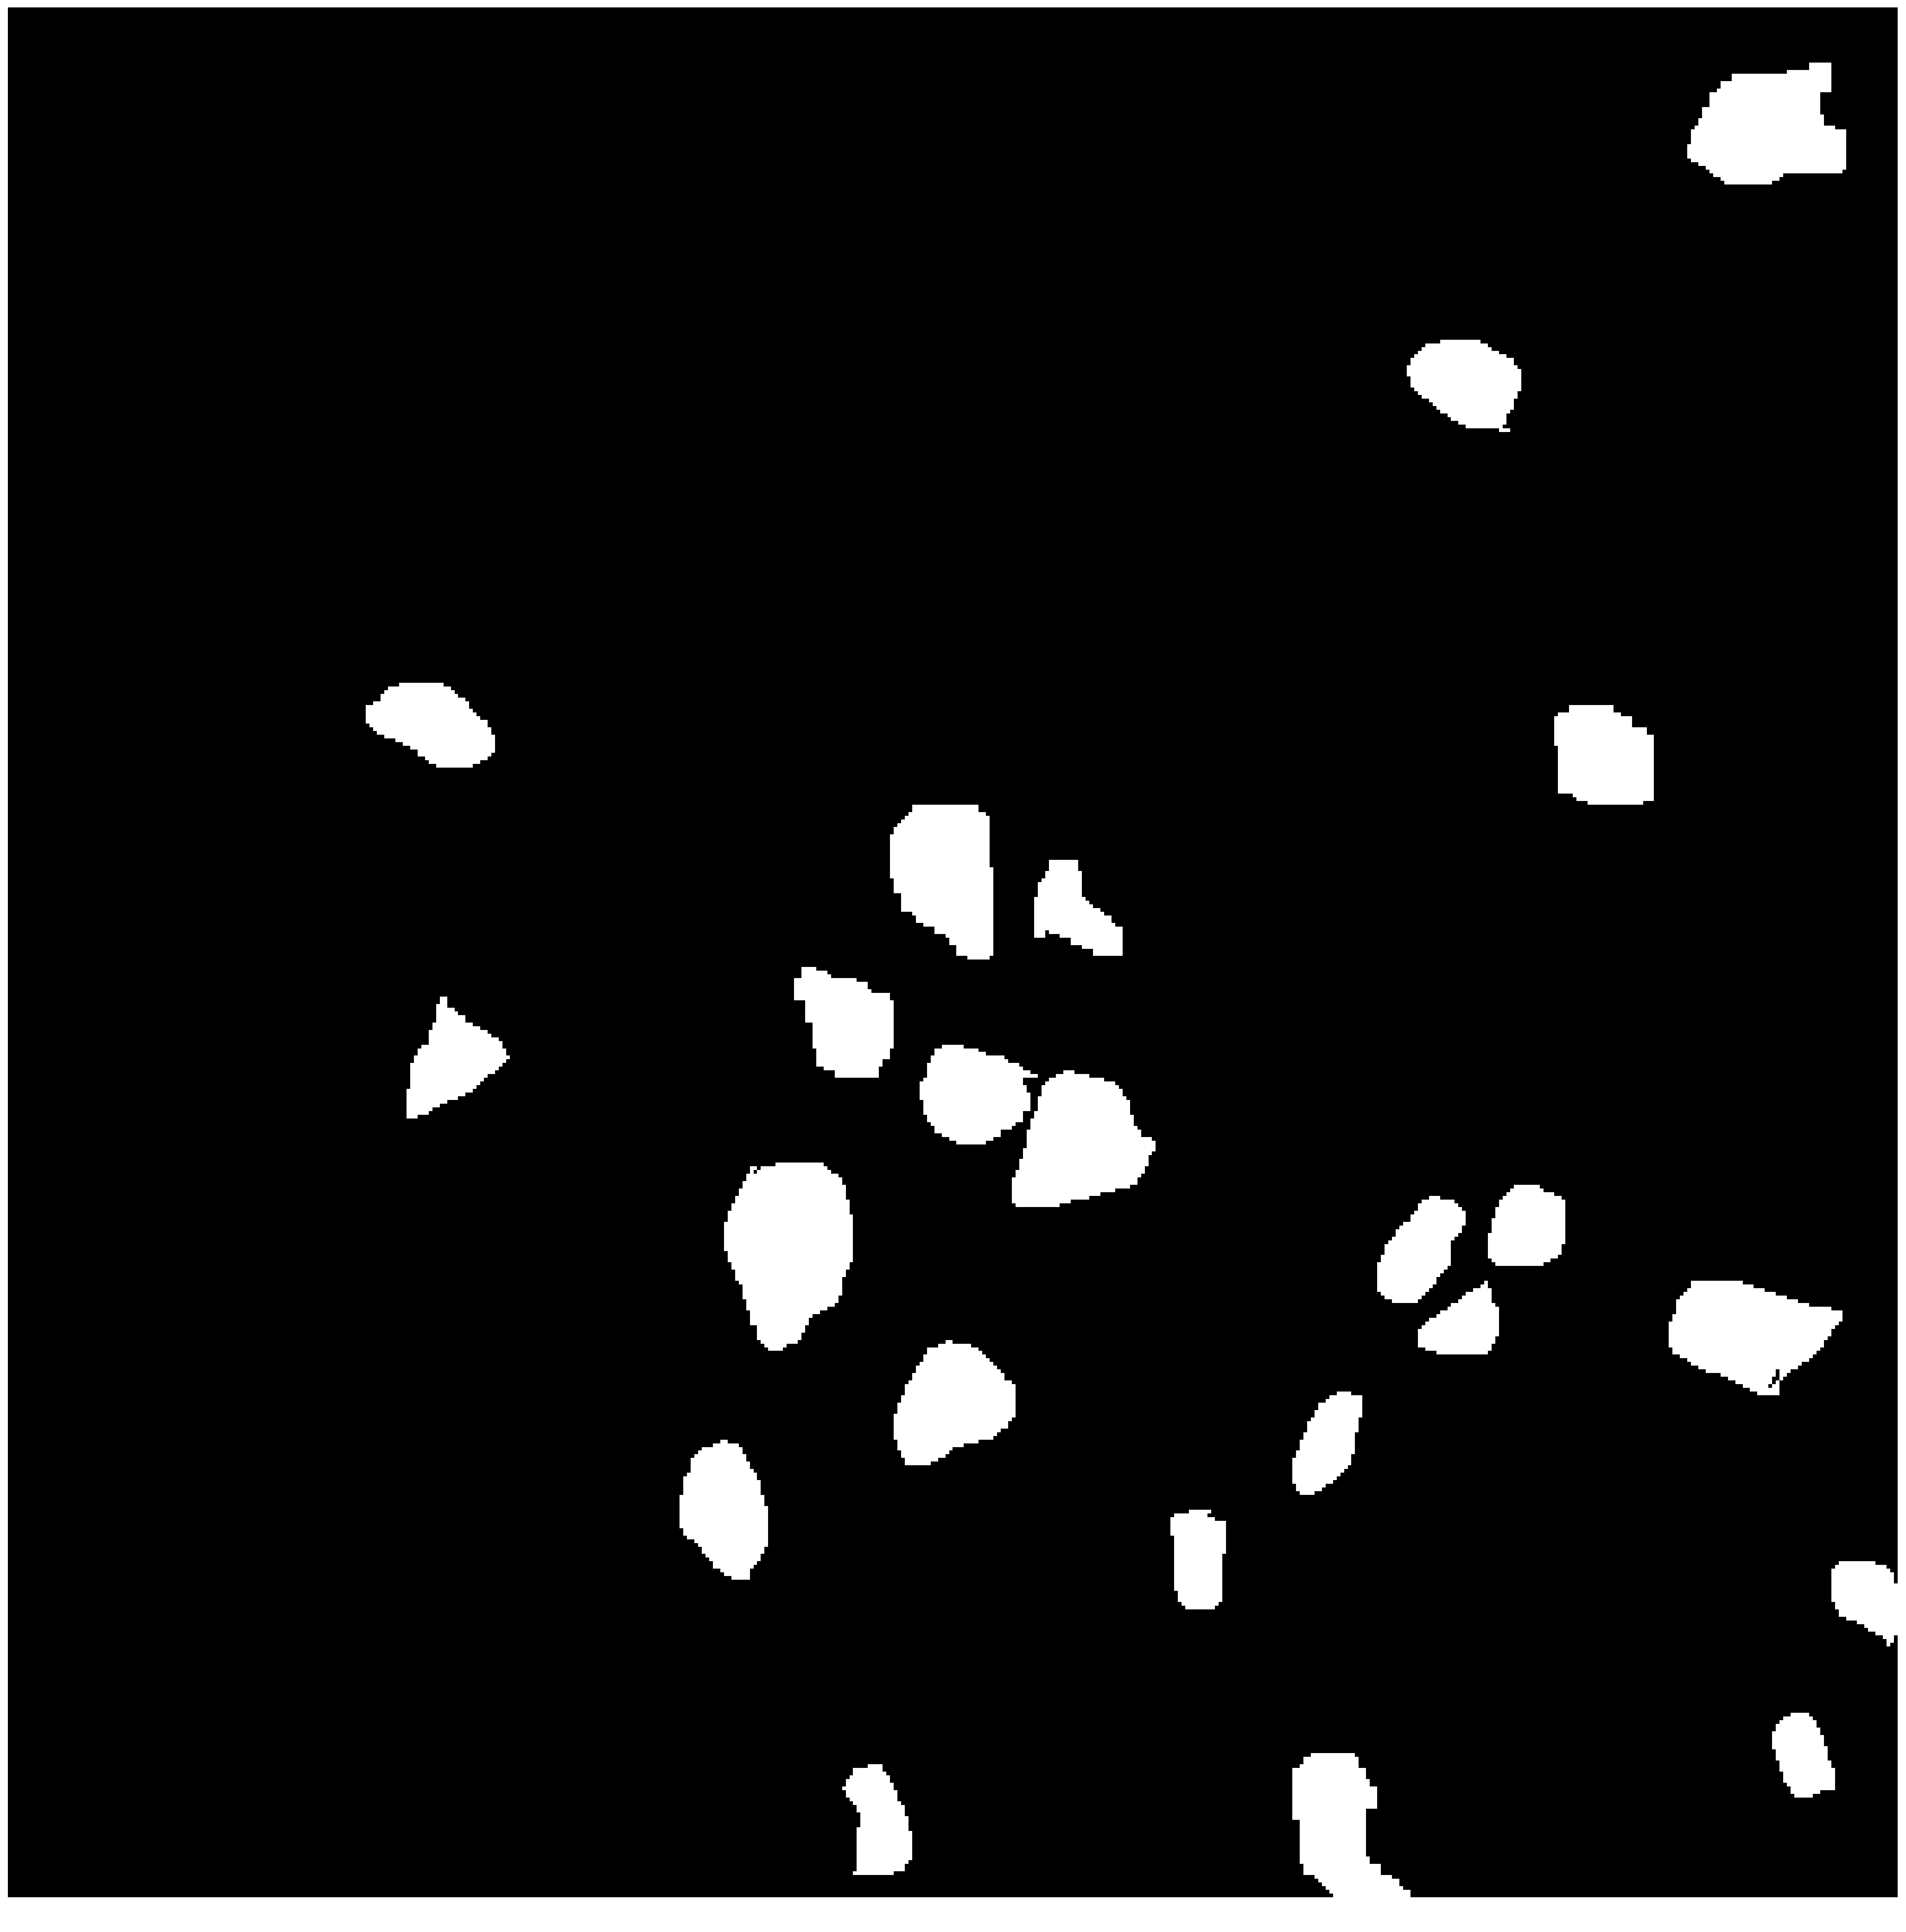
\includegraphics[ width=0.45\textwidth]{figures/130_methods/crop_mask_2451_crop.jpeg}
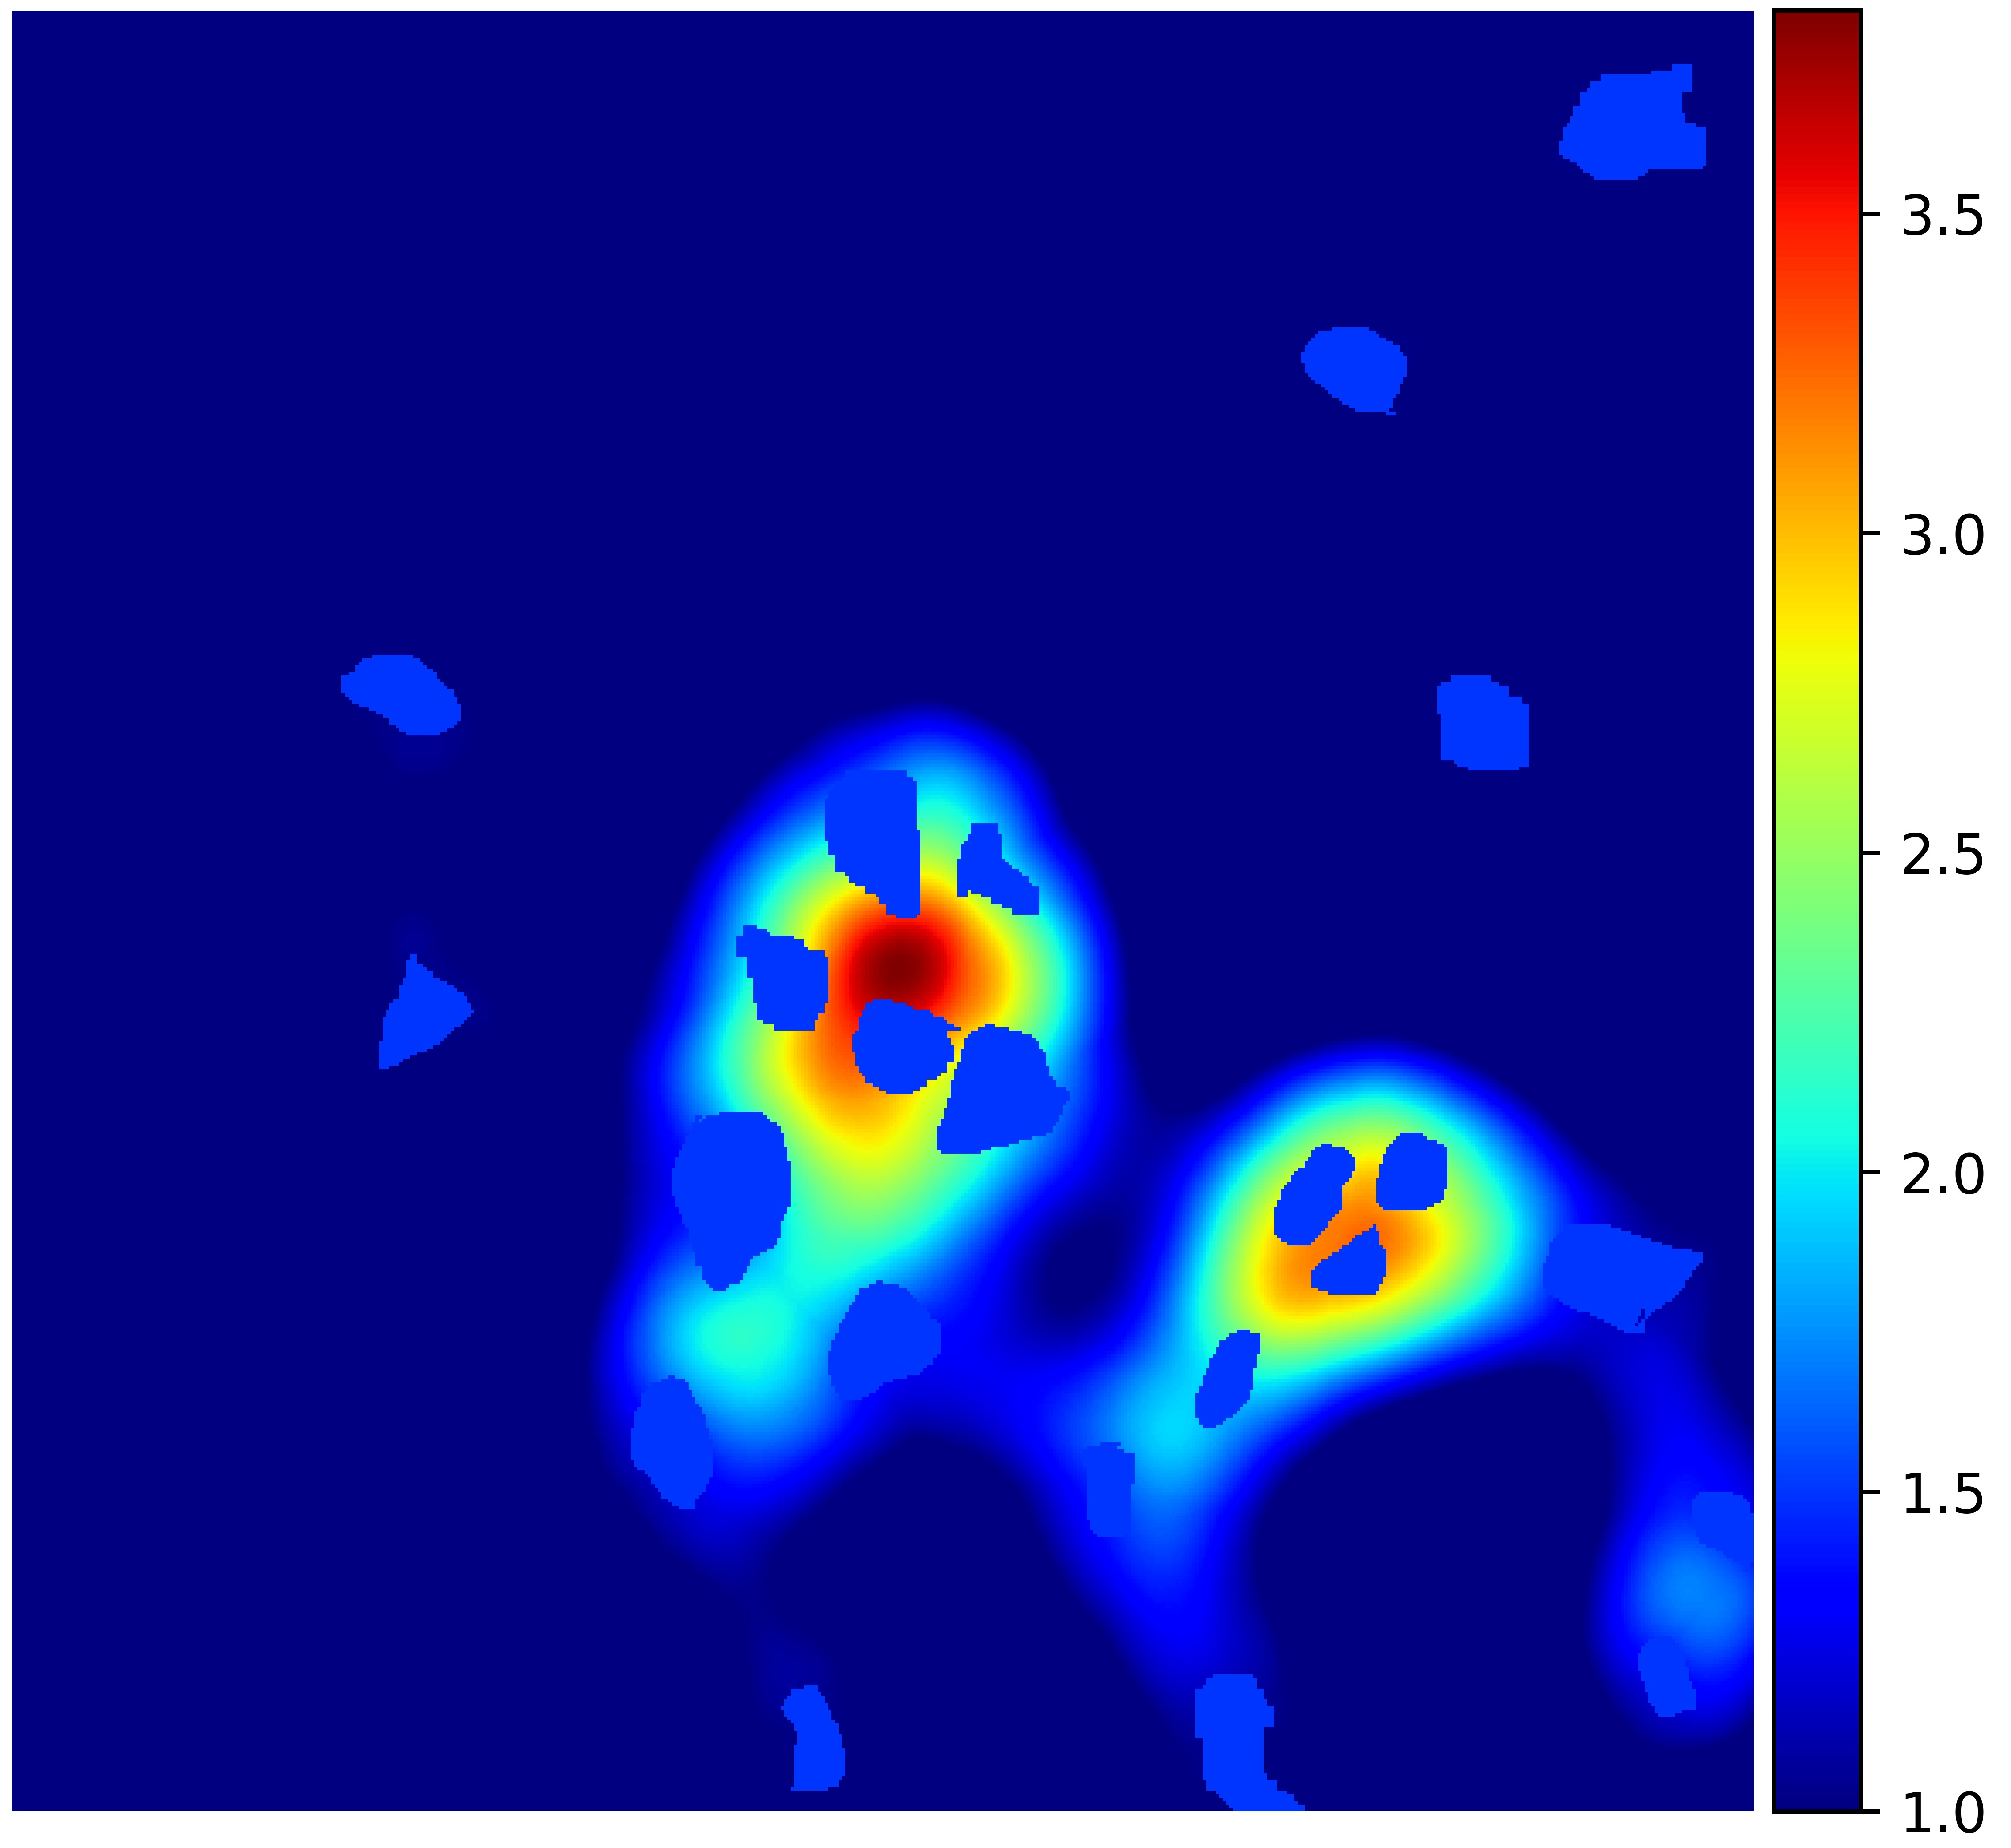
\includegraphics[trim=0 0.008in 0 0, width=0.50\textwidth]{figures/130_methods/crop_weigths_2451_crop.jpeg}
         \caption{Mask and correspondent weight map}
         \label{fig:weight_map_example}
     \end{subfigure}
}
\caption{\textbf{Weight map}. 
\ref{fig:weight_calculation} shows the weight factors of background pixels between cells according to Eq. (\ref{weight_formula}). The dashed curves depict the weights generated by single cells as a function of the distance from their borders.
% , respectively cell 1 on the left (blue) and cell 2 on the right (red).
The green line illustrates the final weight obtained by adding individual contributions. 
In \ref{fig:weight_map_example}, a target mask and the corresponding weight map.} 
\label{fig:weight_map}
\end{figure}
The pseudocode for a weight map is reported in Alg. \ref{algo:pseudocode} 
% (full implementation can be found at $link github$)
, and an example weight map is shown in Fig. \ref{fig:weight_map_example}:

\begin{algorithm}
% \begin{algorithmic}[1]
\DontPrintSemicolon
     Initialize empty $\text{map}_j$ (mask size)\tcp*{weight map $j$-th mask}
    \For{each cell in mask} 
    {
    \tcc{loop over $i$-th cell in $j$-th mask}
         Initialize empty $\text{map}_i$  (mask size) \tcp*{weight map $i$-th cell}
        
         Add $i$-th cell to $\text{map}_i$
        
         Compute euclidean distance between each pixel of $\text{map}_i$ and the closest pixel of the $i$-th cell \label{step:distance}
        
         Compute each pixel's weight in $\text{map}_i$ according to a decreasing exponential function:
        \begin{equation}
        % \hskip 4.5cm
        \text{weight} = \exp\left\{\dfrac{-d^{2}}{2\sigma^{2}}\right\}
        \label{weight_formula}
        \end{equation}
        
        \tcc {$d$ is the distance computed at step \ref{step:distance}}
        \tcc {$\sigma$ is a customizable parameter set to 25 (average cell radius)}
        
    Sum the resulting $\text{map}_i$ to the full $\text{map}_j$
    % , as illustrated in Fig. \ref{fig:weight_calculation};
}
% \end{algorithmic}
\caption{weight map pseudocode for $j$-th mask}
\label{algo:pseudocode}
\end{algorithm}
% \begin{enumerate}
%     \item initialize a completely black image (all pixels with zero value) for the full weight maps;
%     \item initialize a completely black image for the weight map generated by the $i$-th item in the target mask;
%     \item add the $i$-th object to the map created at step 2);
%     \item compute the euclidean distance between each pixel of the current map and the closest pixel belonging to the border of the cell;
%     \item compute the weight attached to each pixel of the map according to a decreasing exponential function:
%         \begin{align}
%         \text{weight} = e^{\frac{-d^{2}}{2\sigma^{2}}}
%         \end{align}
%         \label{weight_formula}
%         where $d$ is the distance computed at step 4) and $\sigma$ is a customizable parameter set to 25 (average cell radius);
%     \item sum the resulting current map to the full weight map, as illustrated in Fig. \ref{fig:weights_formula};
%     \item repeat steps 2) to 6) for each item in the target mask;

% \end{enumerate}

\section{Model training}
\label{sec:model_training}
After randomly setting 70 full-size images apart as a test set, the remaining pictures were randomly split into training and validation sets. 
In particular, twelve 512x512 partially overlapping crops were extracted from each image and fed as input to the network after undergoing a standard augmentation pipeline. Common transformations were considered as rotations, addition of Gaussian noise, brightness variation and elastic transformations \cite{elastic_tranformation}. 
The augmentation factors for crops not included in the artifact oversampling ablation study were set to 10 for manually segmented images and 4 to all the others.
As a result, the model was trained on a total of nearly 16000 images (70\% for training and 30\% for validation).

All competing architectures were trained from scratch under the same conditions to favour a fair comparison.
Specifically, the Adam \cite{adam} optimizer was employed with an initial learning rate of 0.006 and a scheduled decrease of 30\% if the validation loss did not improve for four consecutive epochs. 
A \textbf{weighted binary cross-entropy} loss was adopted on top of the weight maps to handle the unbalance of the two classes (weights equal to 1 and 1.5 for cells and background, respectively).
All models were trained until no improvement was observed for 20 consecutive epochs. In this way, each model was allowed to converge and the comparison was made at the best of each architecture's individual capabilities.

The approach was implemented through Keras API \cite{keras} using TensorFlow \cite{tensorflow} as backend
% and is available at $link _ to _repo$
.
The training was performed on 4 V100 GPUs provided by the \textit{Centro Nazionale Analisi Fotogrammi} (CNAF) computing center of the \textit{National Institute for Nuclear Physics} in Bologna.


\section{Post-processing} \label{sec:post_processing}

\begin{figure}
    \centerline{
    \begin{subfigure}[b]{0.5\textwidth}
        \centering
        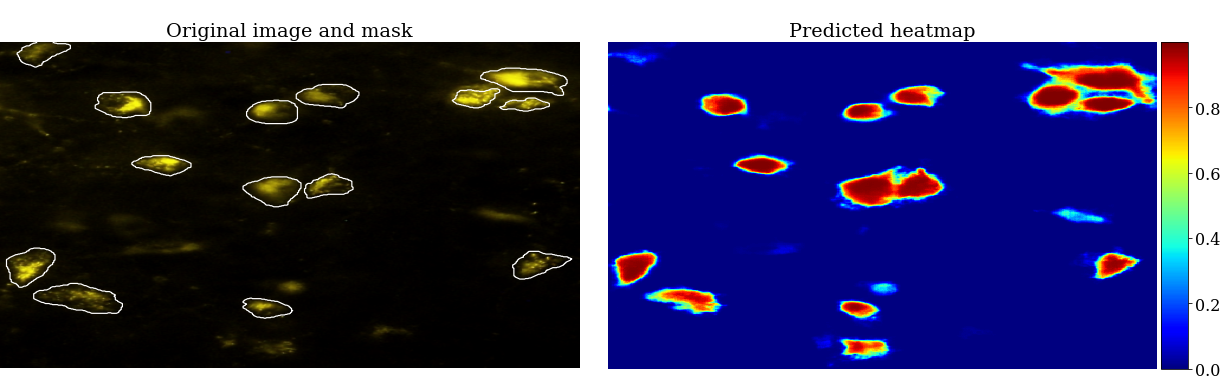
\includegraphics[width=\textwidth]{figures/130_methods/orig+heatmap:278.png}
        \caption{
        % Original image and raw output
        }
        \label{fig:raw_output}
        \end{subfigure}
    \begin{subfigure}[b]{0.5\textwidth}
        \centering
        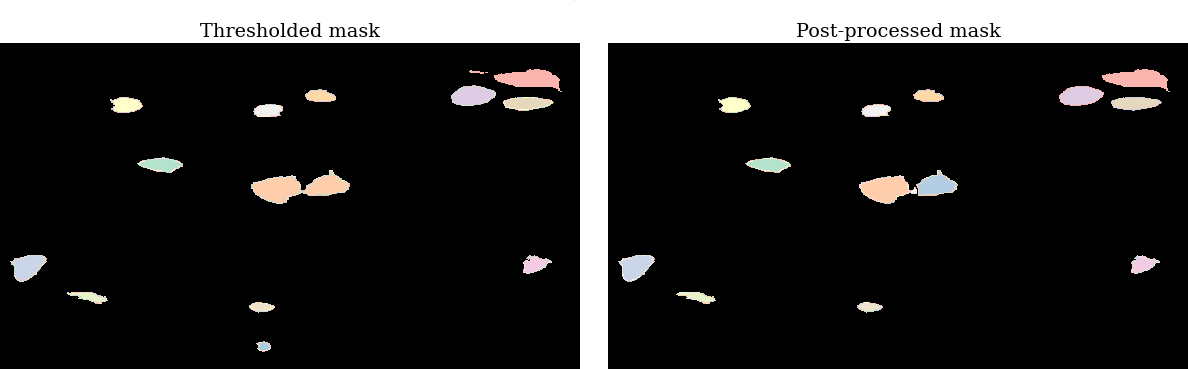
\includegraphics[width=\textwidth]{figures/130_methods/thresh+post_proc:278.png}
        \caption{
        % Thresholded and post-processed predicted masks
        }
        \label{fig:thresh+post_proc}
        \end{subfigure}
    }
    \caption{\textbf{Model output}. 
    From left to right, the input image with white contours indicating annotated cells; the model's raw output (heatmap); 
    the predicted mask after thresholding at 0.875; the predicted mask after post-processing.}
    \label{fig:model_output}
\end{figure}
The final output of the model is a probability map (or heatmap), in which each pixel value represents the probability of belonging to a cell. 
% An example of this outcome is reported on the right of the \ref{fig:raw_output} if the input image on the left is provided to the model.
Fig. \ref{fig:raw_output} reports an example of an input image (left) and the corresponding heatmap (right).
% An example of this outcome is reported in the Fig. \ref{fig:raw_output} (right) if a sample input image (left) is provided to the model.
The higher the value, the higher is the confidence in classifying that pixel as belonging to a cell. 
A thresholding operation was then applied on the heatmap to obtain a binary mask where groups of white connected pixels represent the detected cells. Fig. \ref{fig:thresh+post_proc} (left) illustrates the cells detected after the binarization with different colors.
After that, ad-hoc post-processing was applied to remove isolated components of few pixels and fill the holes inside the detected cells. 
Finally, the watershed algorithm \cite{watershed} was employed with parameters set based on the average cell size.
An example of the results if provided in Fig. \ref{fig:thresh+post_proc}, where the overlapping cells in the middle present in the binary mask (left) are correctly splitted after post-processing (right). Also, the small object in the top right corner is removed
% , and the hole in the bottom right object is filled
.


\section{Model evaluation} \label{sec:model_evaluation}

The Unet, small Unet, ResUnet and c-ResUnet architectures were evaluated and compared based on both detection and counting performance. 
Also, ablation studies assessed the impact of artifacts oversampling and weight maps.

 In order to evaluate the detection ability of the models, a dedicated algorithm was developed.
Specifically, each target cell was compared to all objects in the corresponding predicted mask and uniquely associated with the closest one.
If the distance between their centroids was less than a fixed threshold (50 pixels, i.e. average cell diameter), the predicted element was considered a true positive (TP); a false negative otherwise (FN).
Detected items not associated with any target were considered as false positives (FP) instead.
Starting from these values, we referred to accuracy, precision, recall and $F_1$ score as indicators of detection performance.
% In terms of detection performance, the $F_1$ score was adopted as the primary indicator. Accuracy, precision and recall were also inspected to have a better understanding of the model ability. 
The definitions of such metrics are reported below:

\begin{align}
% \hskip 2cm
\text{accuracy} &=  \frac{\text{TP}}{\text{TP} + \text{FP} + \text{FN}}
= \frac{\text{1}}{\text{1} + \frac{1}{\text{TP}} \left(\text{FP} + \text{FN}\right)}
\label{eq:accuracy}; \\ 
\text{precision} &=    \frac{\text{TP}}{\text{TP} + \text{FP}}; \\
\text{recall} &=    \frac{\text{TP}}{\text{TP} + \text{FN}}; \\ 
F_1 \text{score} &=  \frac{2 * \text{precision} * \text{recall}}{\text{precision} + \text{recall}}
= \frac{2*\text{TP}}{2*\text{TP} + \text{FP} + \text{FN}} 
= \frac{\text{1}}{\text{1} + \frac{1}{\text{2TP}} \left(\text{FP} + \text{FN}\right)}
\label{eq:F1}.
\end{align}
% where TP, FP and FN indicates true positive (cells correctly detected), false positives (cells erroneously detected) and false negatives (cells erroneously missed), respectively. 
Notice that we do not have true negatives in Eq. \eqref{eq:accuracy} since the prediction of the class "not cell" is done at the pixel level and not at the object level, so there are no "non-cell" objects predicted by the model.

Regarding the counting task, the Mean Absolute Error (MAE), Median Absolute Error (MedAE) and Mean Percentage Error (MPE) were used instead. More precisely, let $n_{\text{pred}}$ be the number of detected cells in $i$-th image  and $n_{\text{true}}$ be the actual one. Then, the absolute error (AE) and the percentage error (PE) were defined as:

\begin{align}
% \hskip 2cm
\text{AE} &= \lvert n_{\text{true}} - n_{\text{pred}}\rvert ;\\
\text{PE} &= \frac{ n_{\text{true}} - n_{\text{pred}}}{n_{\text{true}} 
% + \epsilon
}.
\end{align}
% where $\epsilon=10^{-6}$ was added to prevent a vanishing denominator when $n_{\text{true}} = 0$. 
Hence, the above counting metrics are just the mean and the median of the AE and the PE.
% The $F_1$ score was adopted for measuring the detection performance, while Mean Absolute Error (MAE), Median Absolute Error (MedAE) and Mean Percentage Error (MPE) were used as counting metrics. 

% The choice of the optimal cutoff for binarization was made based on the $F_1$ score computed on full-size images. 
% Although the ultimate goal is retrieving the counts, we relied on detection performance to enforce accurate recognition and avoid spurious balancing between false positives and false negatives that are indistinguishable from the counts.
% Also, full-size images (and not crops) are used to simulate better the model's performance in a real-world scenario.

\noindent\textbf{Threshold optimization}.
% In practice, a dedicated algorithm was developed to determine the correctness of model predictions.
% Specifically, each target cell was compared to all objects in the corresponding predicted mask and uniquely associated with the closest one.
The choice of the optimal cutoff for binarization was made based on the $F_1$ score computed on full-size images. In practice, each model was evaluated on a grid of values and the best one was selected according to the \textit{Kneedle} method \cite{kneedle}. The resultant threshold was then used to assess performances on the test set.
Although the ultimate goal is retrieving the counts, we relied on detection performance to enforce accurate recognition and avoid spurious balancing between false positives and false negatives that are indistinguishable from the counts.
Also, full-size images (and not crops) are used to simulate better the model's performance in a real-world scenario.
\begin{figure}
\centerline{
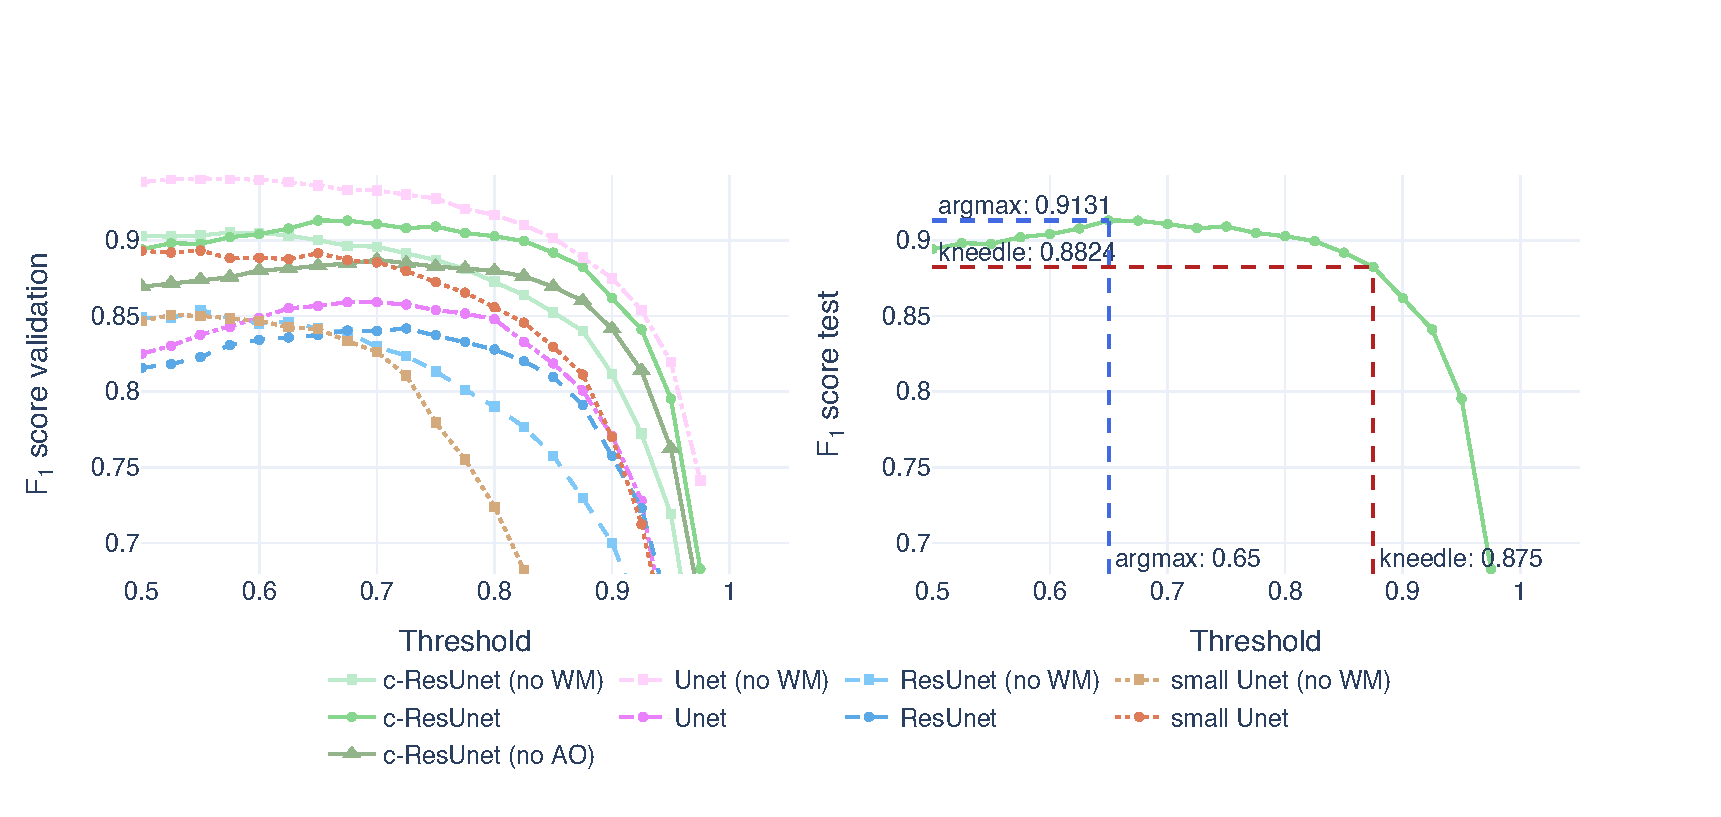
\includegraphics[width=0.8\linewidth]{figures/130_methods/F1_optimization.eps}
}
\caption{\textbf{Threshold optimization}. On the left, the $F_{1}$ score computed on validation images as a function of the cutoff for thresholding.
On the right, the test $F_1$ score of the c-ResUnet model is used to illustrate the selection of the best threshold for binarization according to \textit{argmax} (blue) and \textit{kneedle} (red) methods.
} 
\label{fig:thresh_opt}
\end{figure}
% If the distance between their centroids was less than a fixed threshold (50 pixels, i.e. average cell diameter), the predicted element was considered a true positive; a false negative otherwise.
% Detected items not associated with any target were considered as false positives instead.

Figure \ref{fig:thresh_opt} shows the optimization results. On the left, we can see how each model performance varies in the validation set as a function of the cutoff for binarization.
Even though lower thresholds work best for all models, the $F_1$ curves are rather flat after their peaks. Thus, increasing the cutoff allows focusing only on predictions whereby the model is very confident, with just a slight loss in overall performance.
Also, good practices in natural science applications suggest being conservative with counts and only consider clearly stained cells.
For these reasons, we resorted to the \textit{Kneedle} method \cite{kneedle} for the selection of the optimal threshold. An example of that choice in the case of c-ResUnet is reported in Figure \ref{fig:thresh_opt} (right plot).
